\section{日本全国の結果}
\label{sec:japan}

\subsection{冬の気球はどこへ流されるか}

冬の日本の上空には強い西風（ジェット気流）が吹いている。標準の飛行では、
どこから上げても平均で東へ約 \SI{255}{\kilo\metre} 流される（図~\ref{fig:drift}）。
南へ行くほどジェットの芯に近く、流される距離が長い。

このため、打ち上げ地点の\textbf{東 \SIrange{150}{350}{\kilo\metre}} に目標が広がっているかどうかで
結果がほぼ決まる。九州北西部から上げると、その先に瀬戸内海が東西 \SI{400}{\kilo\metre} にわたって
横たわっている。瀬戸内海は冬でも雪がなく、落下点がそこに入れば成功に数える。
これが西日本の北西部が有利になる理由である。

\begin{figure}[htbp]
\centering
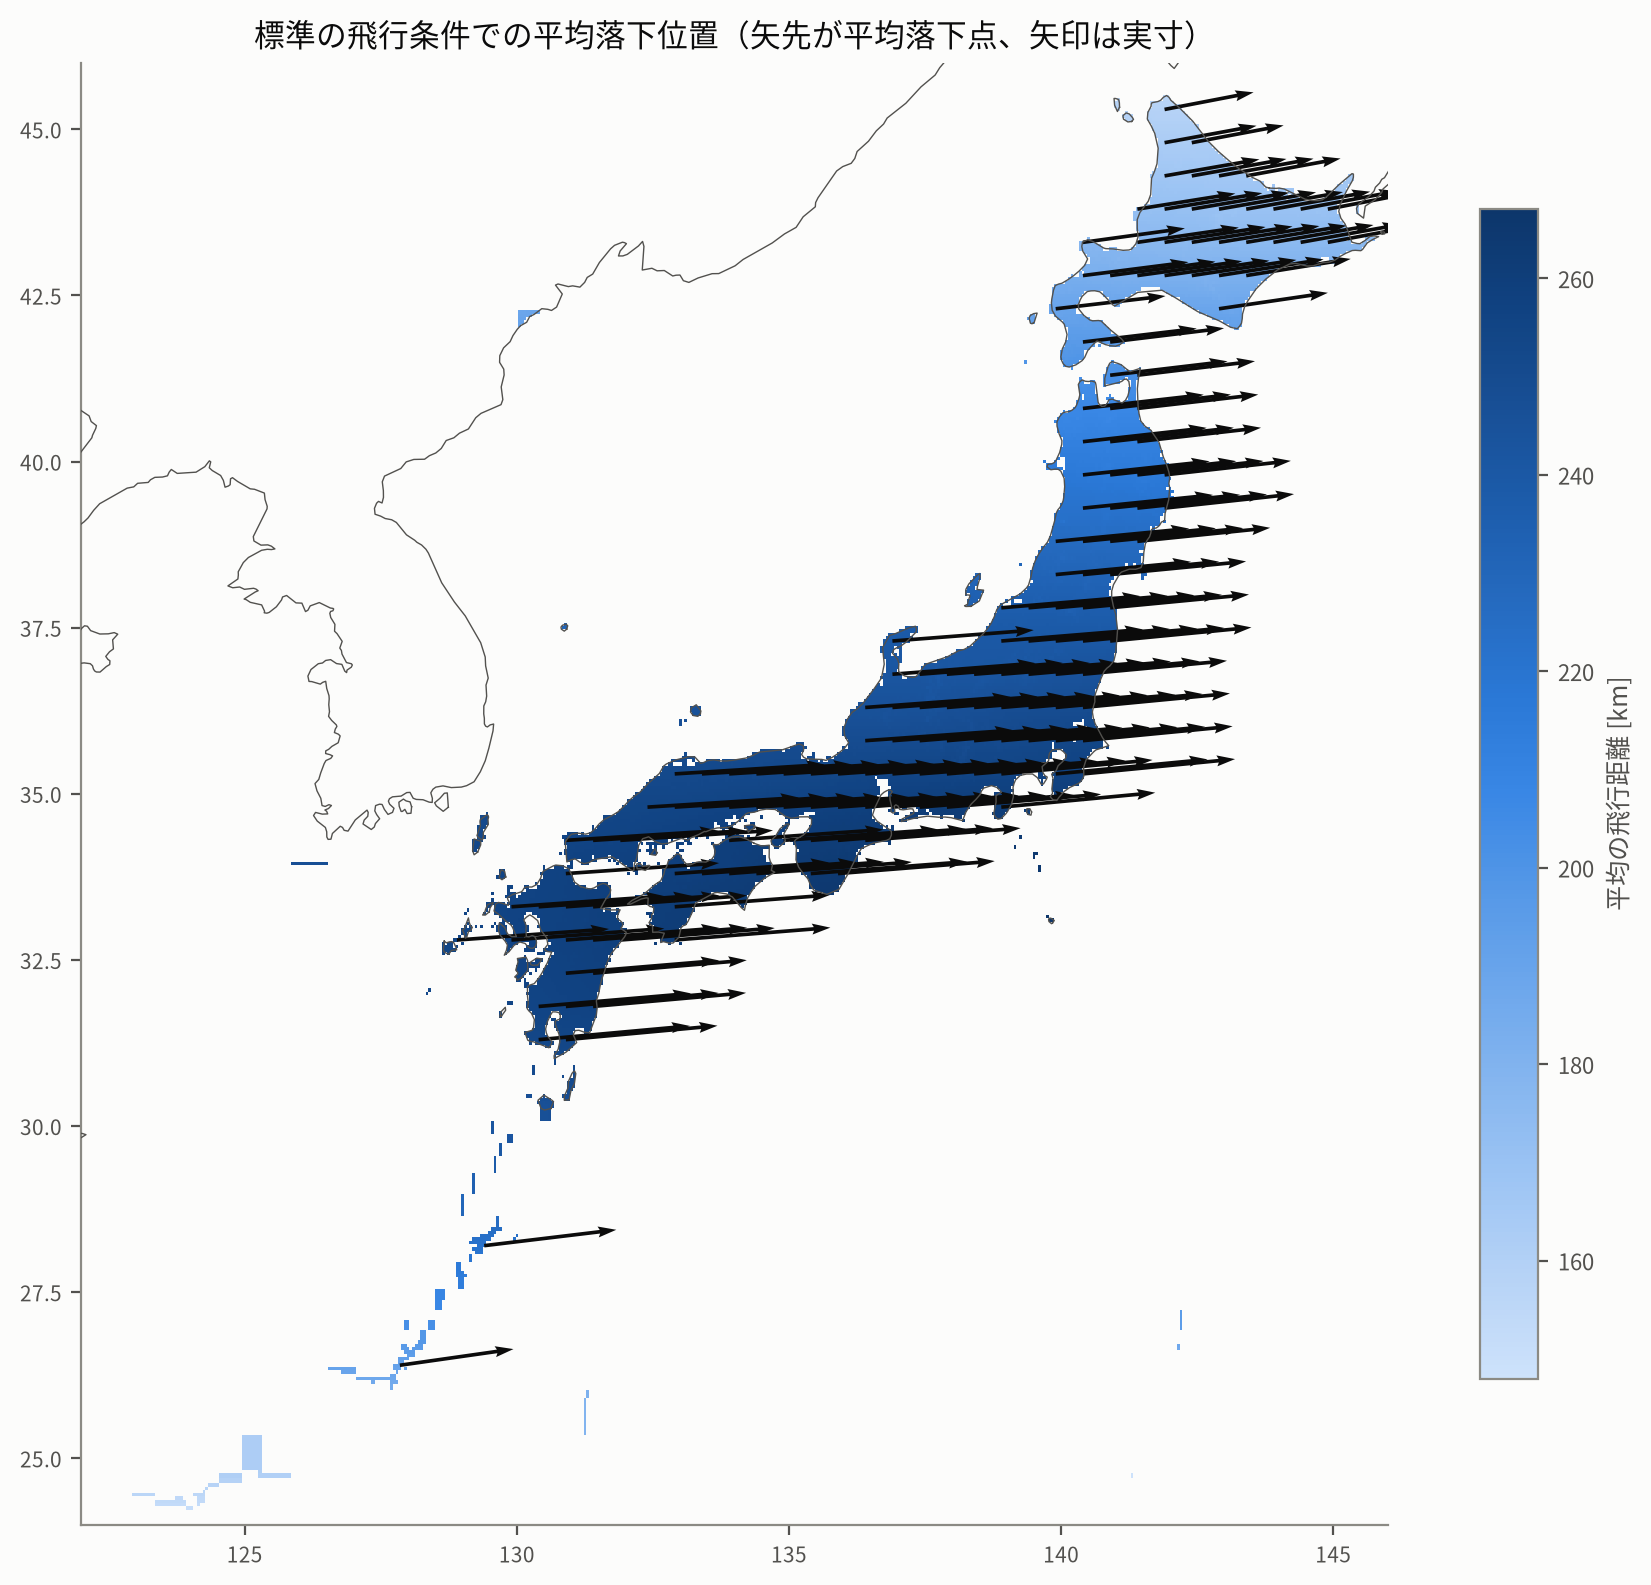
\includegraphics[width=\linewidth]{drift_arrows.png}
\caption{標準の飛行での平均落下位置（903 日の平均）。矢印は実寸で、根元が打ち上げ地点、
矢先が平均の落下点。色は平均の飛行距離。}
\label{fig:drift}
\end{figure}

\subsection{実施できる確率の地図}

図~\ref{fig:pmaps} は、全候補について 4 つの確率を地図にしたものである。
「落下予測が目標に入る」確率（左上）は、九州北西部と山口県で \SIrange{40}{50}{\percent} ある。
ここに雪（右上）と地上気象（左下）の条件を重ねると、実施できる確率（右下）は
最も高い場所でも \SI{33}{\percent} になる。

\begin{figure}[htbp]
\centering
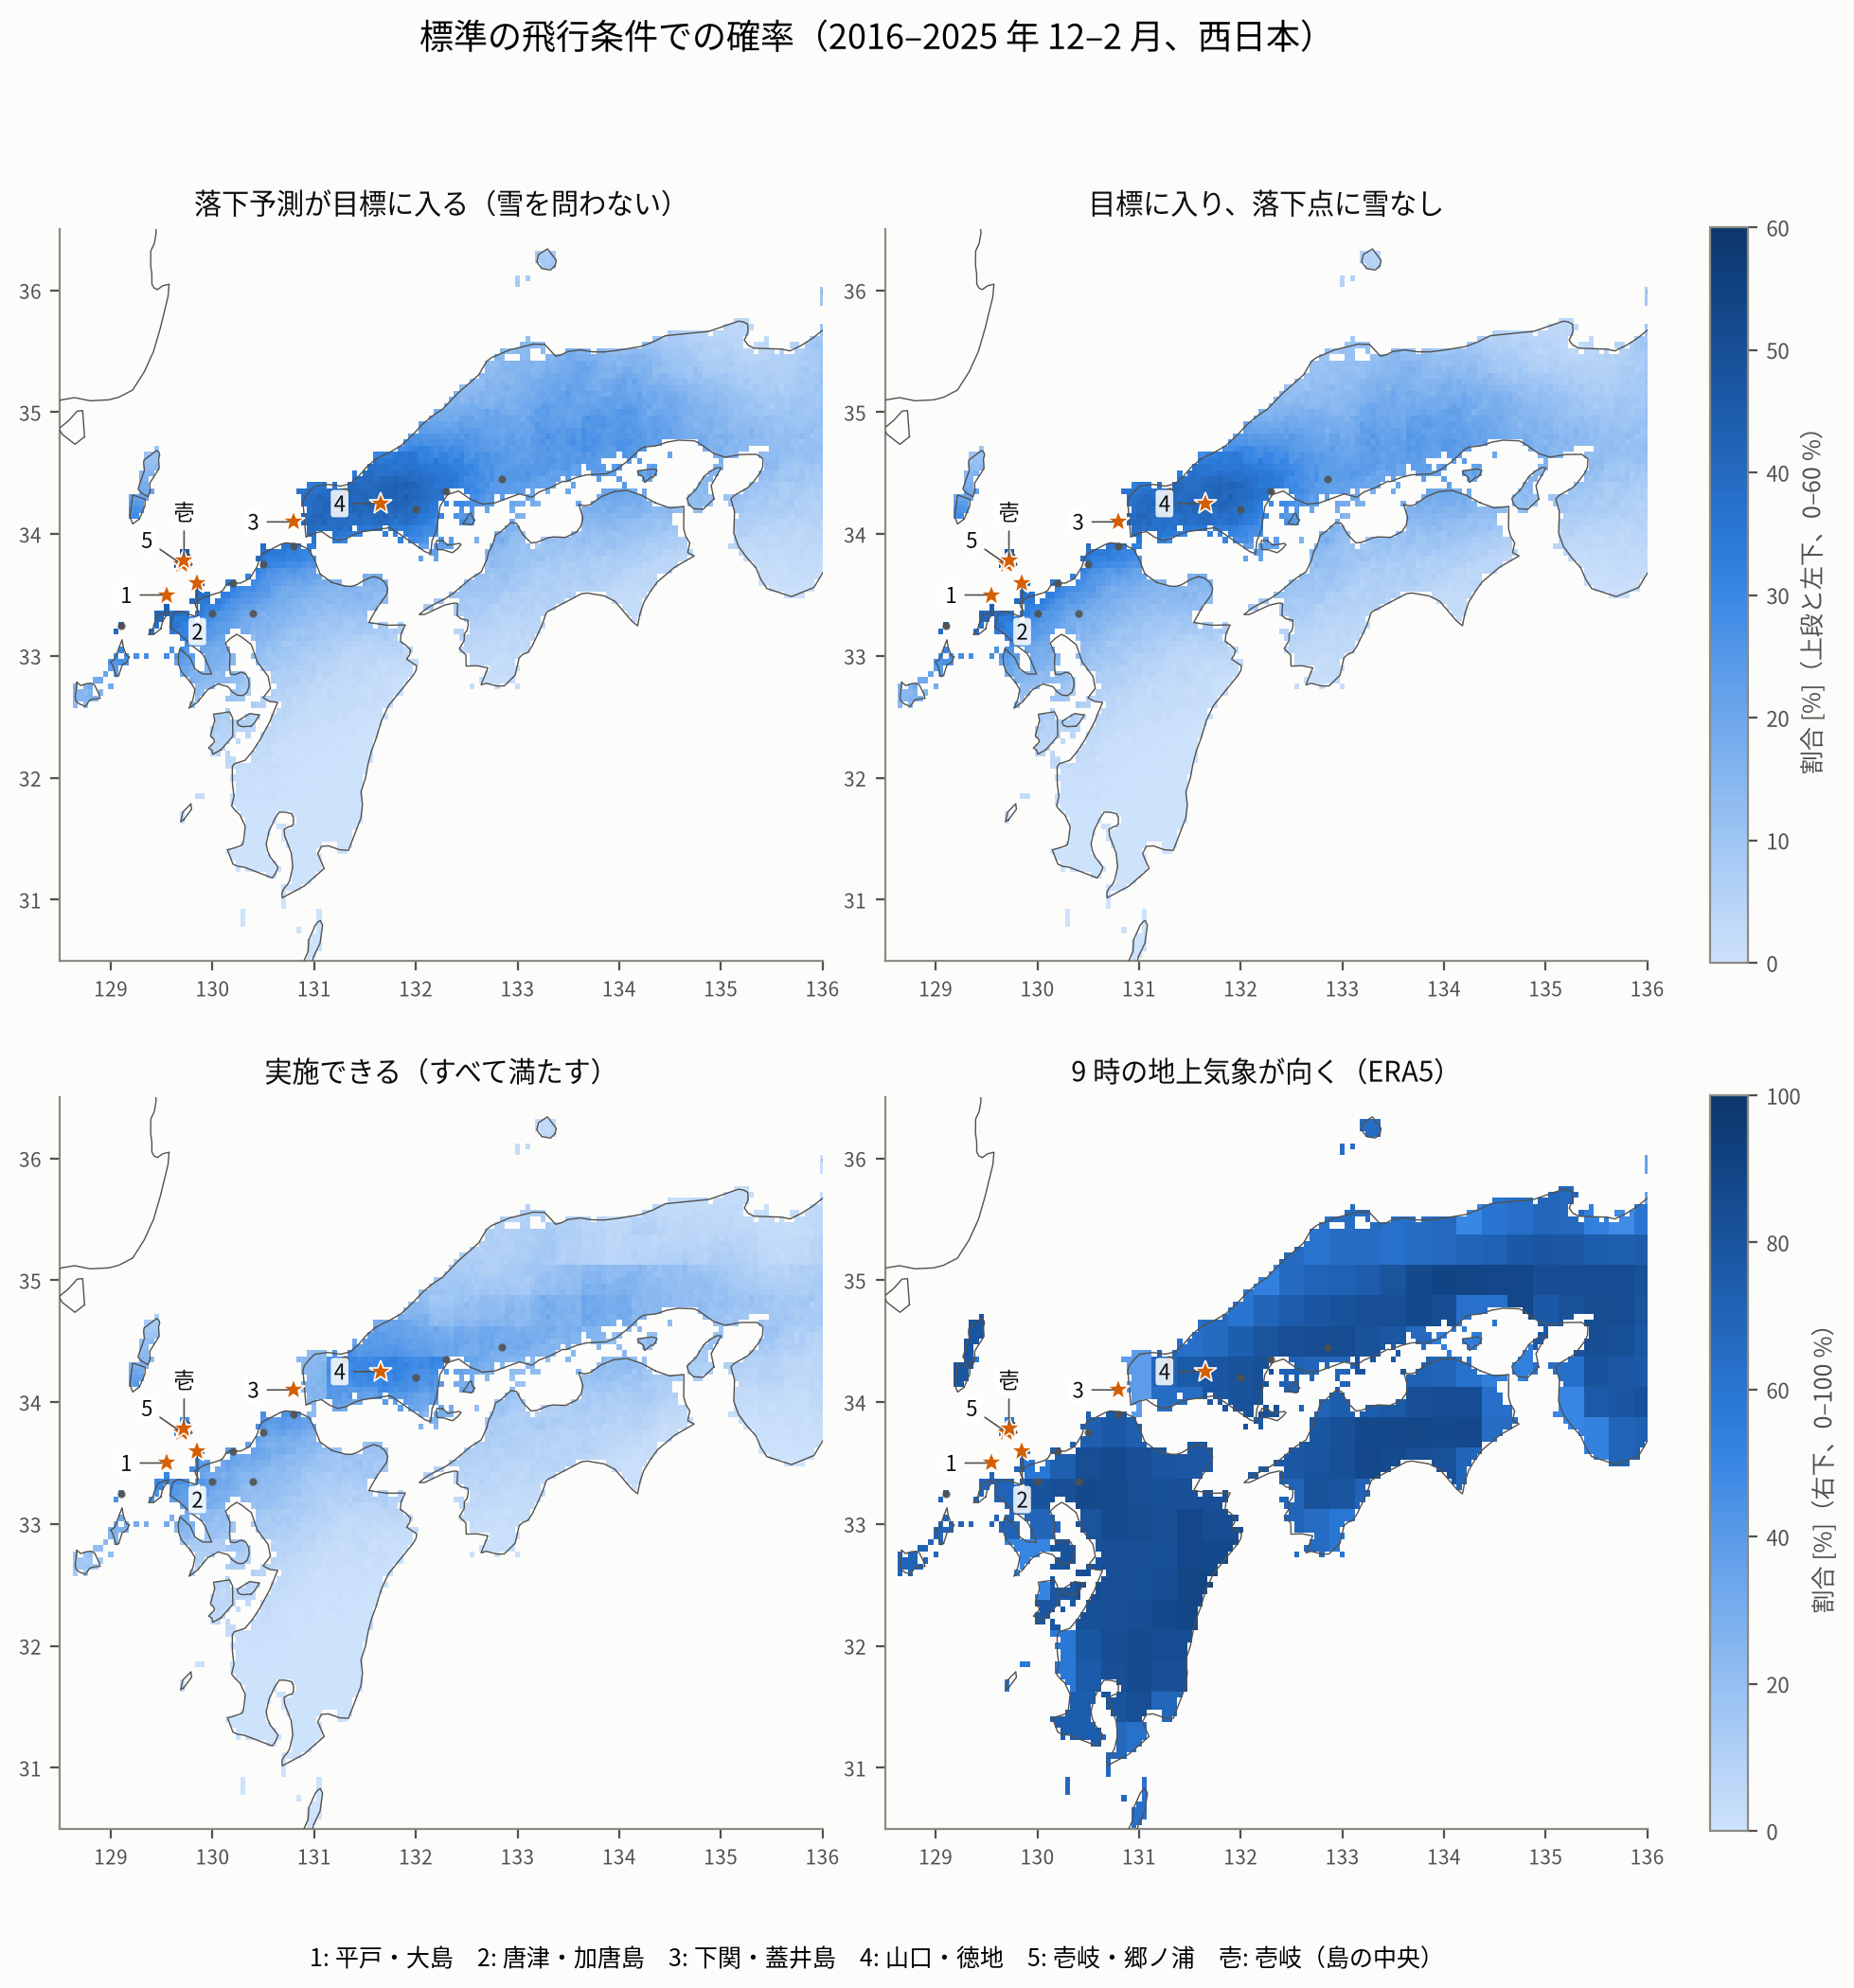
\includegraphics[width=\linewidth]{p_maps_std.png}
\caption{標準の飛行での確率。左上: 落下予測が目標に入る（雪を問わない）。
右上: 加えて落下点に雪がない。左下: 9 時の地上気象が向く。右下: すべてを満たす（実施できる）。
番号は上位の候補地。}
\label{fig:pmaps}
\end{figure}

地方ごとに最も高い地点を表~\ref{tab:region} にまとめた。北海道・東北は打ち上げ地点の雪で、
関東は落下点が太平洋の沖に出るため、ほとんど実施できない。
短時間の飛行にすると、飛行距離が縮んで中国地方や四国の瀬戸内海側でも瀬戸内海・
平野に落ちるようになり、各地の確率が上がる（図~\ref{fig:pshort}）。

\begin{table}[htbp]
\centering
\small
\caption{地方ごとの最も高い地点（打ち上げ地点の標高 \SI{200}{\metre} 以下、飛行条件のばらつきなし）。}
\label{tab:region}
\begin{tabular}{lcrcr}
\toprule
& \multicolumn{2}{c}{標準の飛行} & \multicolumn{2}{c}{短時間の飛行} \\
地方 & 地点 & 実施 [\%] & 地点 & 実施 [\%] \\
\midrule
北海道 & 42.80, 143.20 & 3 & 43.15, 143.65 & 5 \\
東北 & 37.80, 139.10 & 2 & 37.95, 139.10 & 4 \\
関東 & 36.25, 138.90 & 5 & 36.25, 138.90 & 20 \\
中部・東海 & 35.50, 137.05 & 27 & 35.30, 138.45 & 25 \\
近畿 & 34.85, 134.50 & 15 & 34.75, 134.85 & 27 \\
四国 & 34.00, 132.15 & 23 & 34.40, 133.00 & 37 \\
中国 & 34.35, 131.30（長門） & 32 & 34.45, 132.85（東広島） & 44 \\
九州・壱岐・対馬 & 33.50, 129.55（平戸・大島） & \textbf{33} & 33.60, 130.20（糸島） & \textbf{51} \\
南西諸島 & 24.45, 122.95 & 5 & 26.35, 126.80 & 13 \\
\bottomrule
\end{tabular}
\end{table}

\begin{figure}[htbp]
\centering
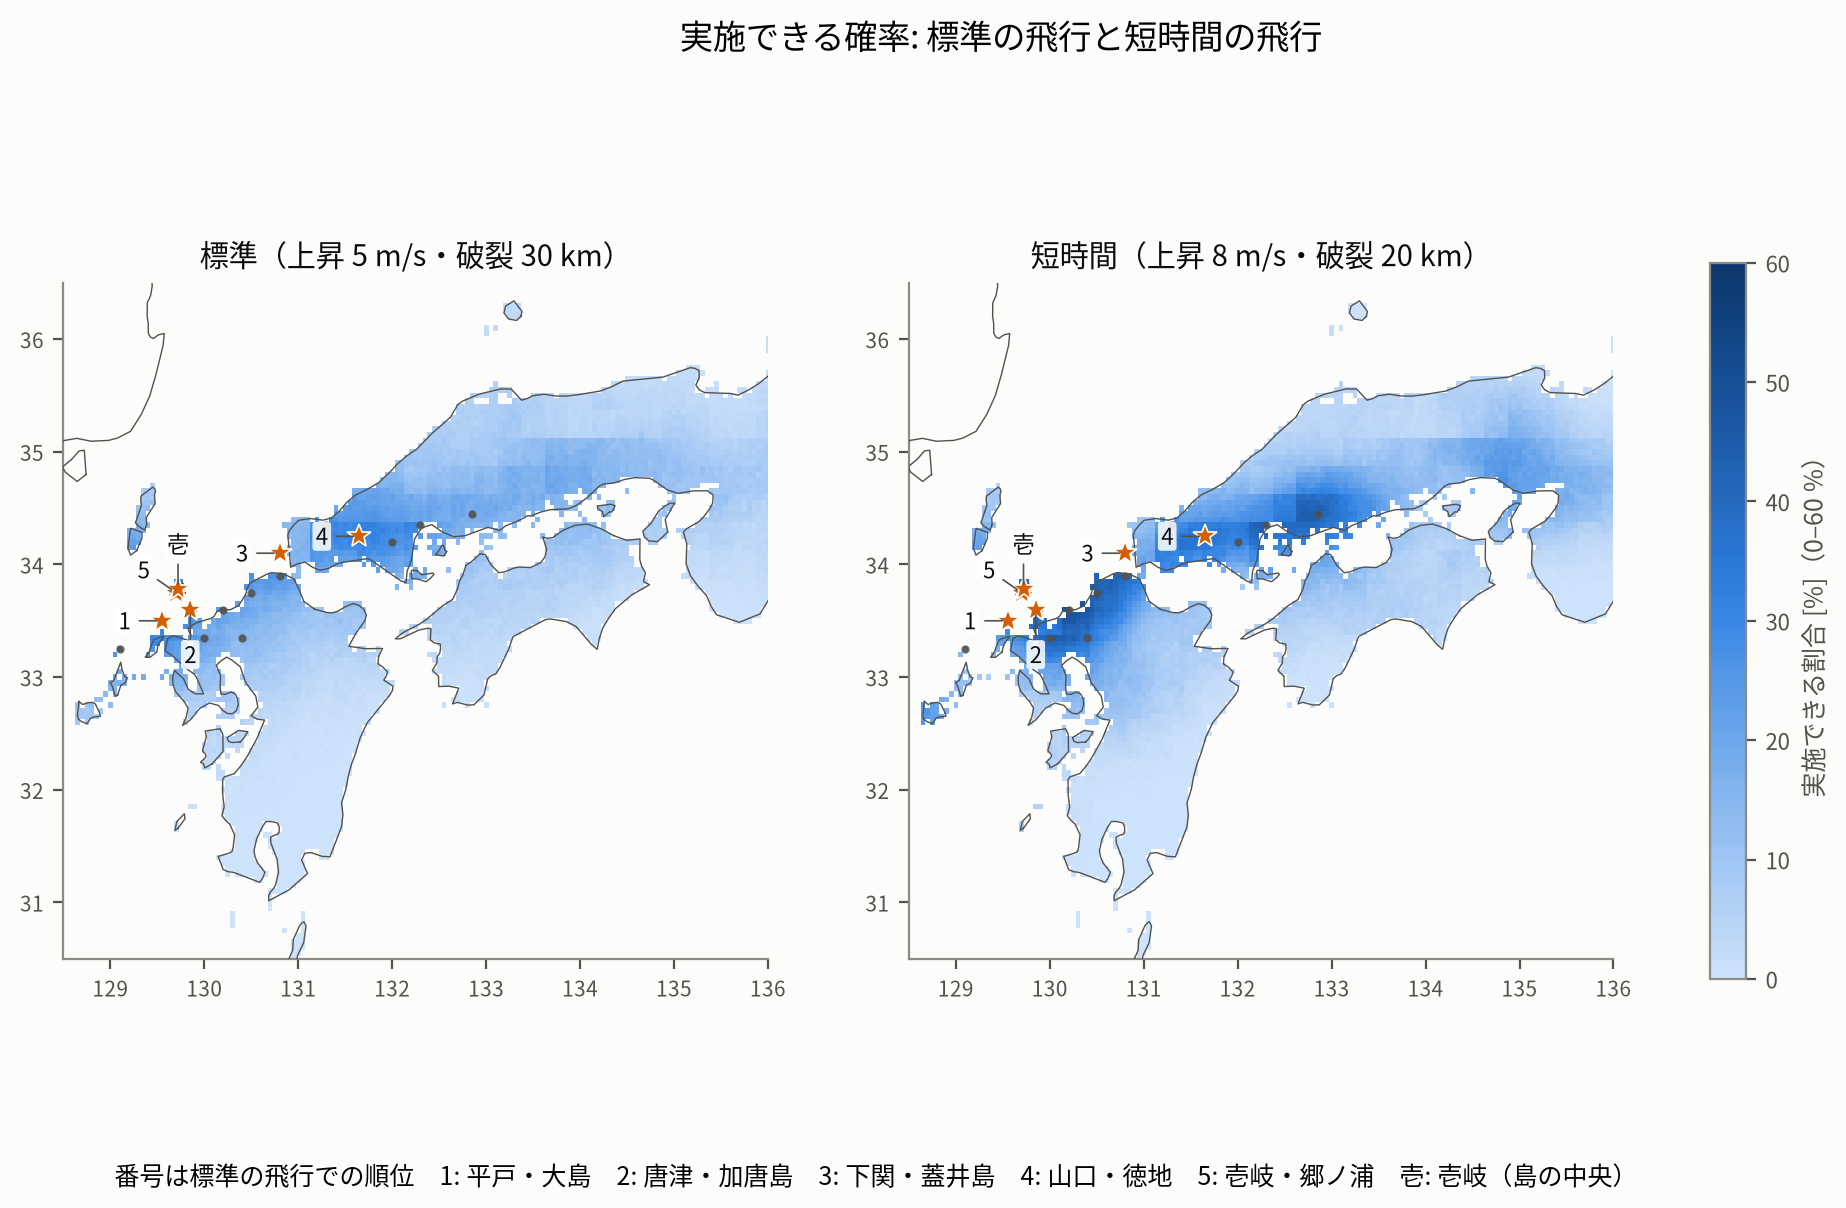
\includegraphics[width=\linewidth]{p_maps_short.png}
\caption{実施できる確率の比較。左が標準の飛行、右が短時間の飛行。}
\label{fig:pshort}
\end{figure}

\begin{figure}[htbp]
\centering
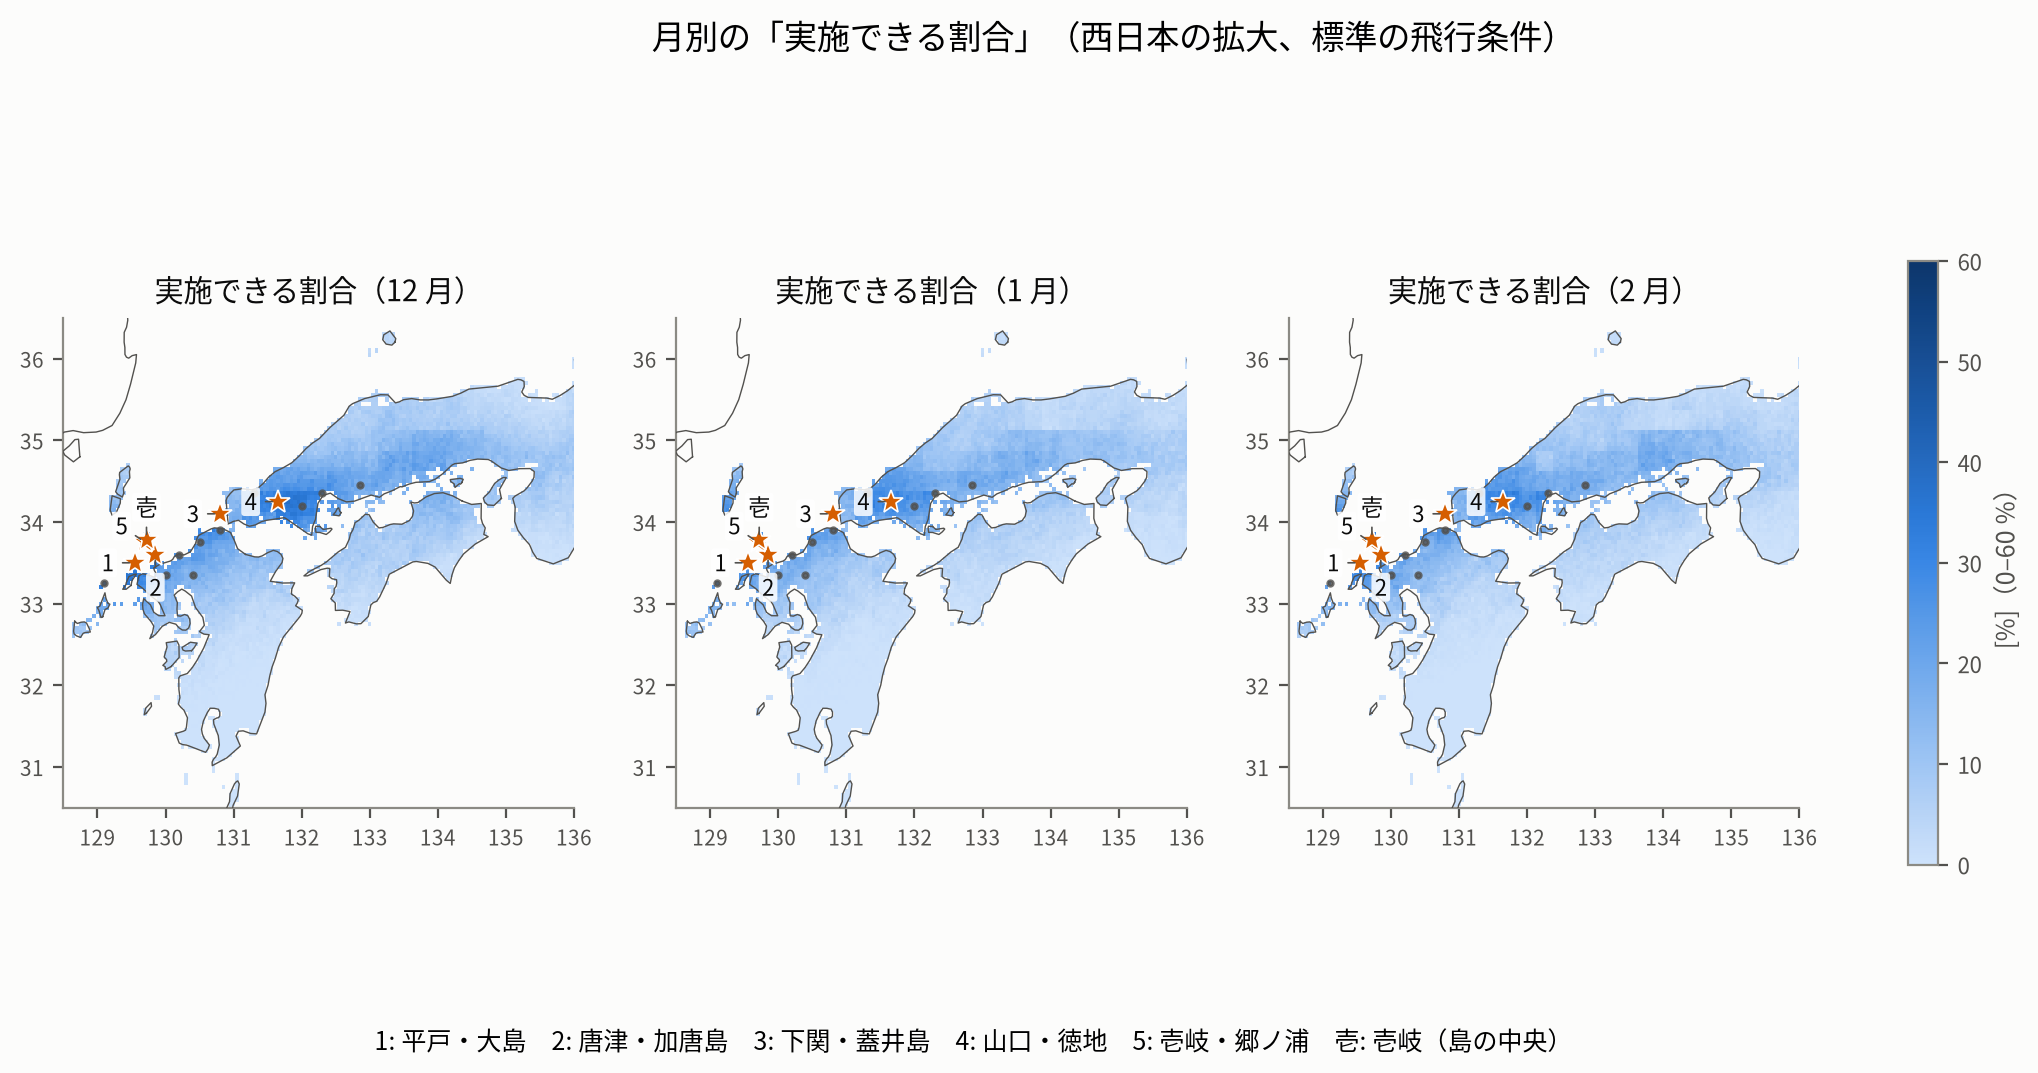
\includegraphics[width=\linewidth]{p_total_months.png}
\caption{標準の飛行で実施できる確率の月ごとの違い。}
\label{fig:months}
\end{figure}
